\documentclass[10pt]{article}

\usepackage[paperwidth=8.5in, paperheight=11in, margin=1in]{geometry}
\usepackage{booktabs}
\usepackage{graphicx}
\usepackage[export]{adjustbox}
\usepackage{array}
\usepackage{float}
\pagenumbering{gobble}
\usepackage{caption}
\captionsetup[table]{skip=10pt}

% \renewcommand{\familydefault}{\sfdefault}
\usepackage{fontspec}
\setmainfont{Times New Roman}
\setlength\parindent{0pt}

\renewcommand{\thefigure}{S\arabic{figure}}
\renewcommand{\thetable}{S\arabic{table}}

\begin{document}

\begin{figure}
  \centering
  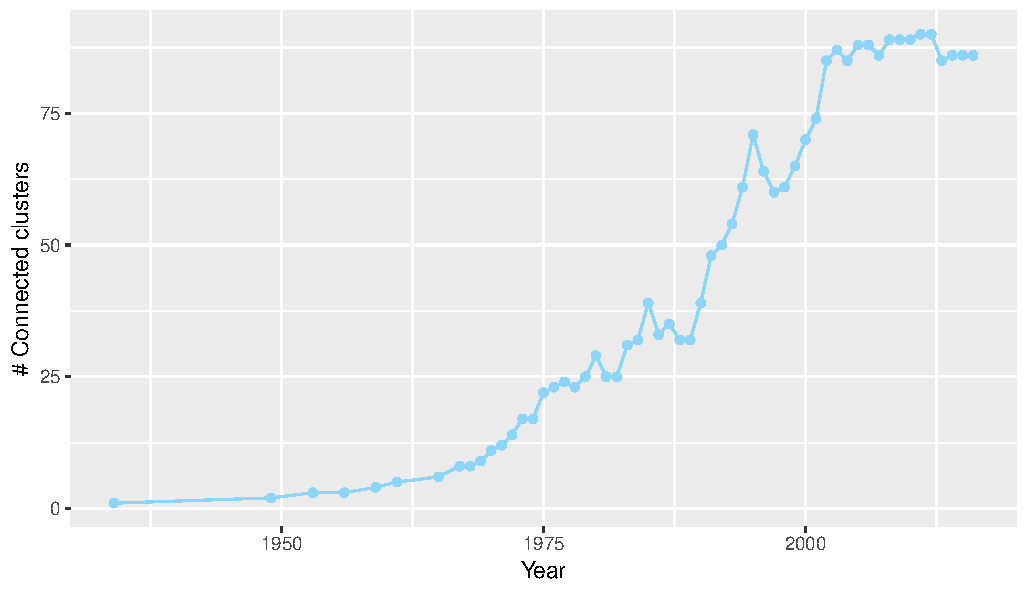
\includegraphics[width=0.9\textwidth]{../S1/FigureS1.pdf}
  \caption{Number of connected components per year.}
  \label{fig:s1}
\end{figure}

\begin{figure}
  \centering
  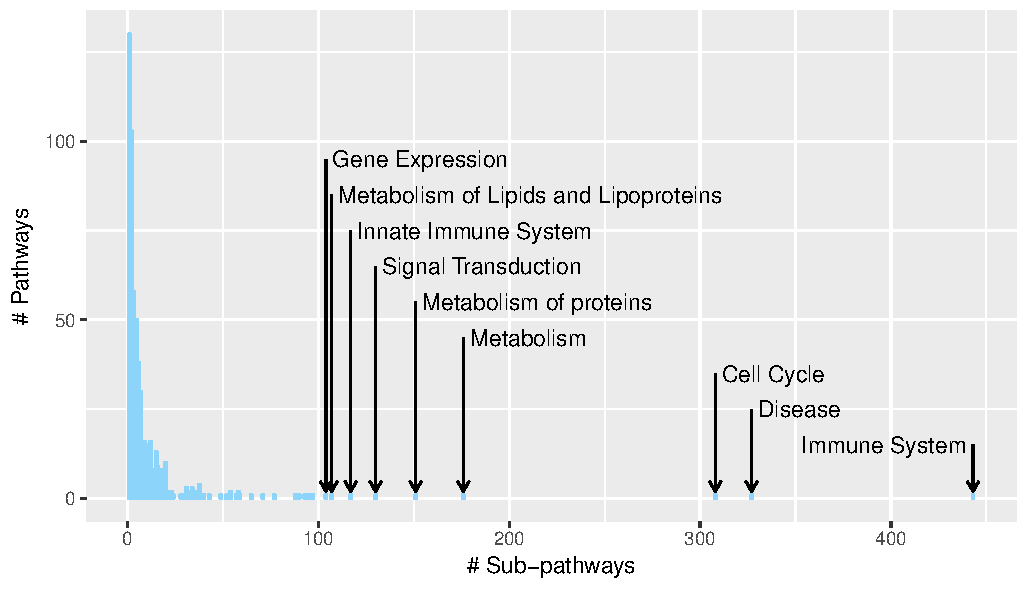
\includegraphics[width=0.9\textwidth]{../S2/FigureS2.pdf}
  \caption{Distribution of the number of sub-pathways for all
    pathways. There are 2051 pathways annotated in total. Most
    pathways (1397) do not contain any sub-pathways. Of the remaining
    650, most contain few sub-pathways. The nine pathways with more
    than 100 sub-pathways are annotated in the plot. Innate Immune
    System is a sub-pathway of Immune System, Metabolism of Lipids and
    Lipoproteins is a sub-pathway of Metabolism, the other pathways
    are all top-level pathways.}
  \label{fig:s2}
\end{figure}

\begin{figure}
  \centering
  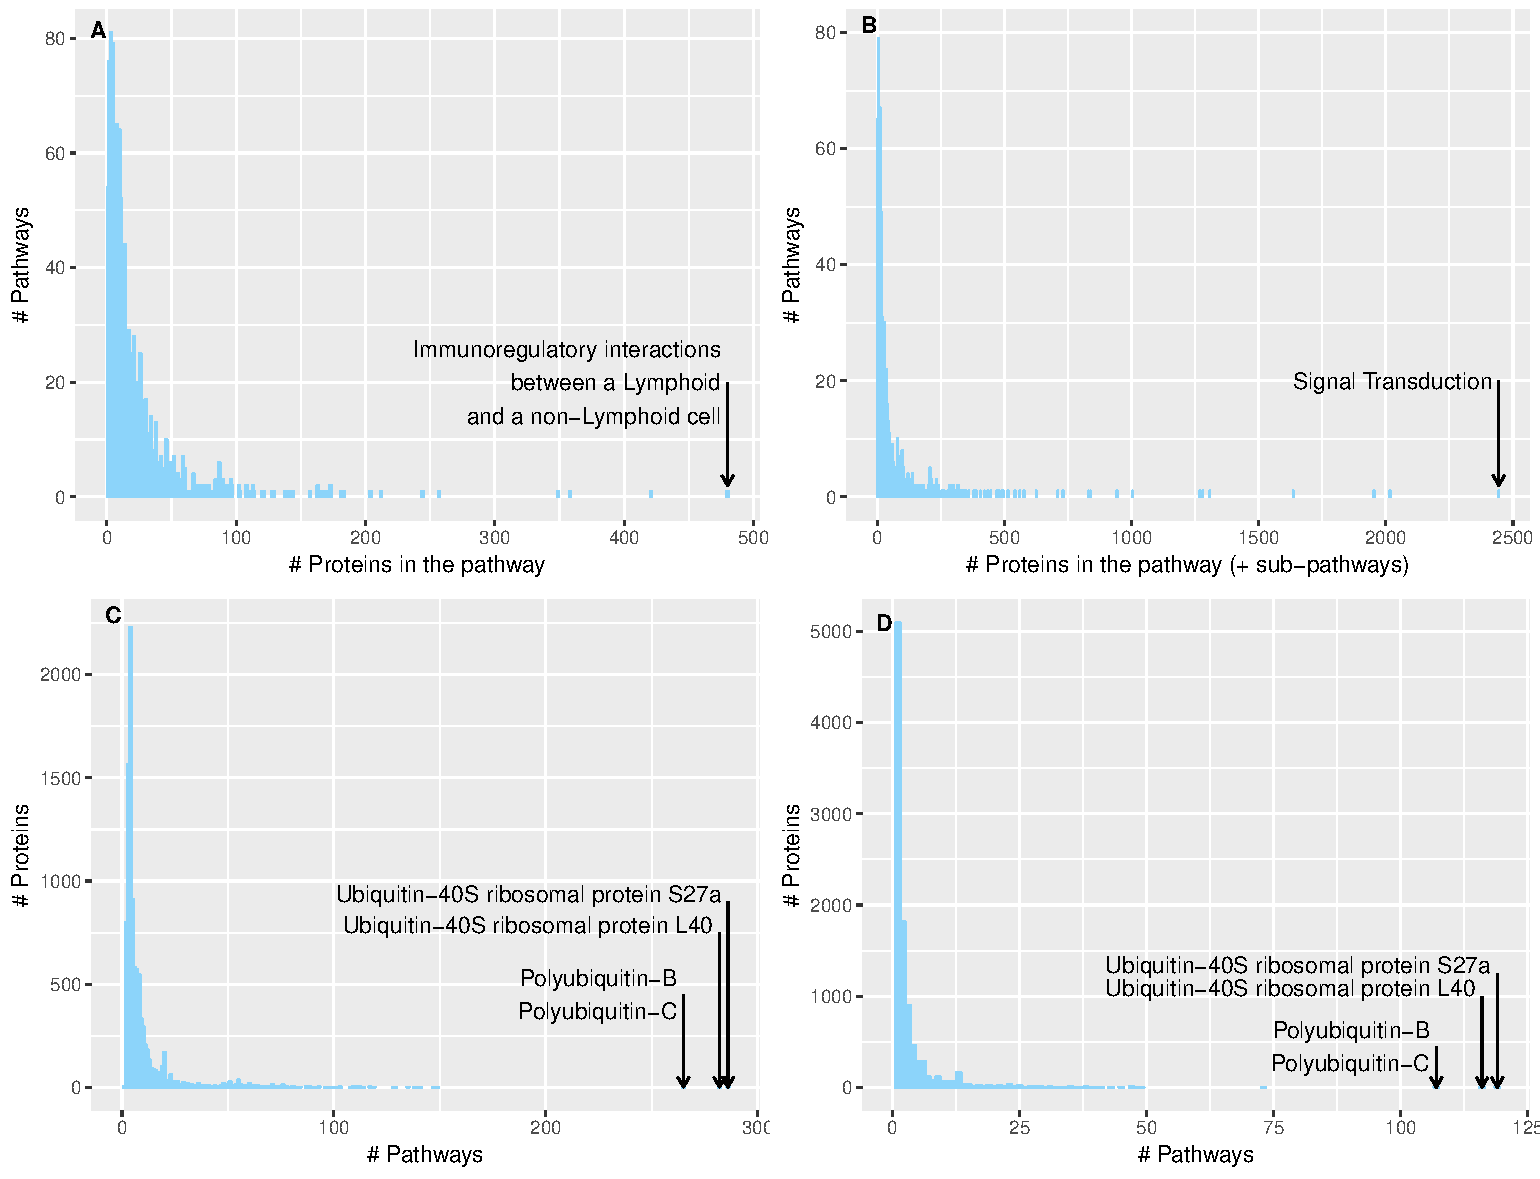
\includegraphics[width=0.9\textwidth]{../S3/FigureS3.pdf}
  \caption{Number of proteins per pathway and vice versa. A) Number of
    proteins directly occurring in each pathway. B) Number of proteins
    occurring in each pathway, including the proteins occurring in
    sub-pathways. C) Number of pathways a protein occurs in, including
    the pathways where the protein occurs in a sub-pathway. D) Number
    of pathways a protein directly occurs in.}
  \label{fig:s3}
\end{figure}

\begin{figure}
  \centering
  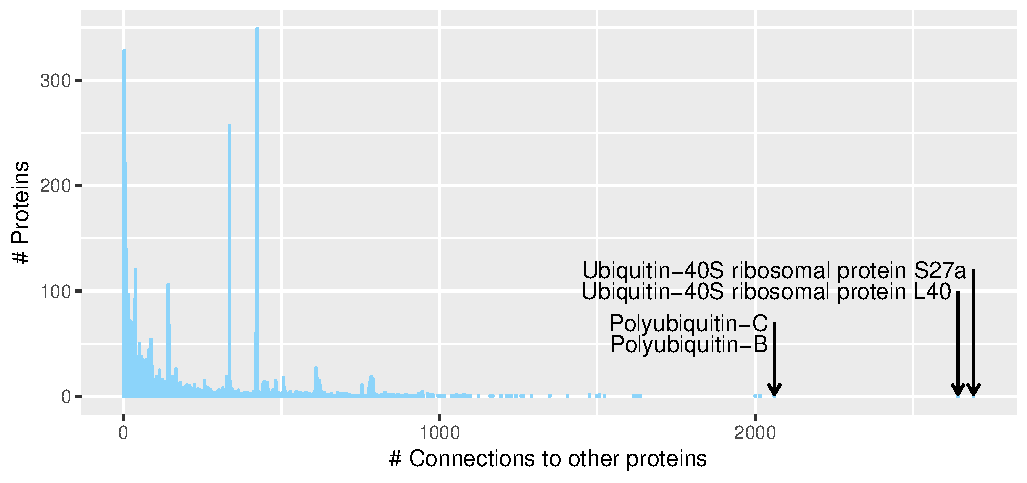
\includegraphics[width=0.9\textwidth]{../S4/FigureS4.pdf}
  \caption{Distribution of the number of connections for each protein.
    The two big spikes around 400 connections are mainly olfactory
    receptors and zinc fingers. 
  }
  \label{fig:s4}
\end{figure}


\begin{figure}
  \centering
  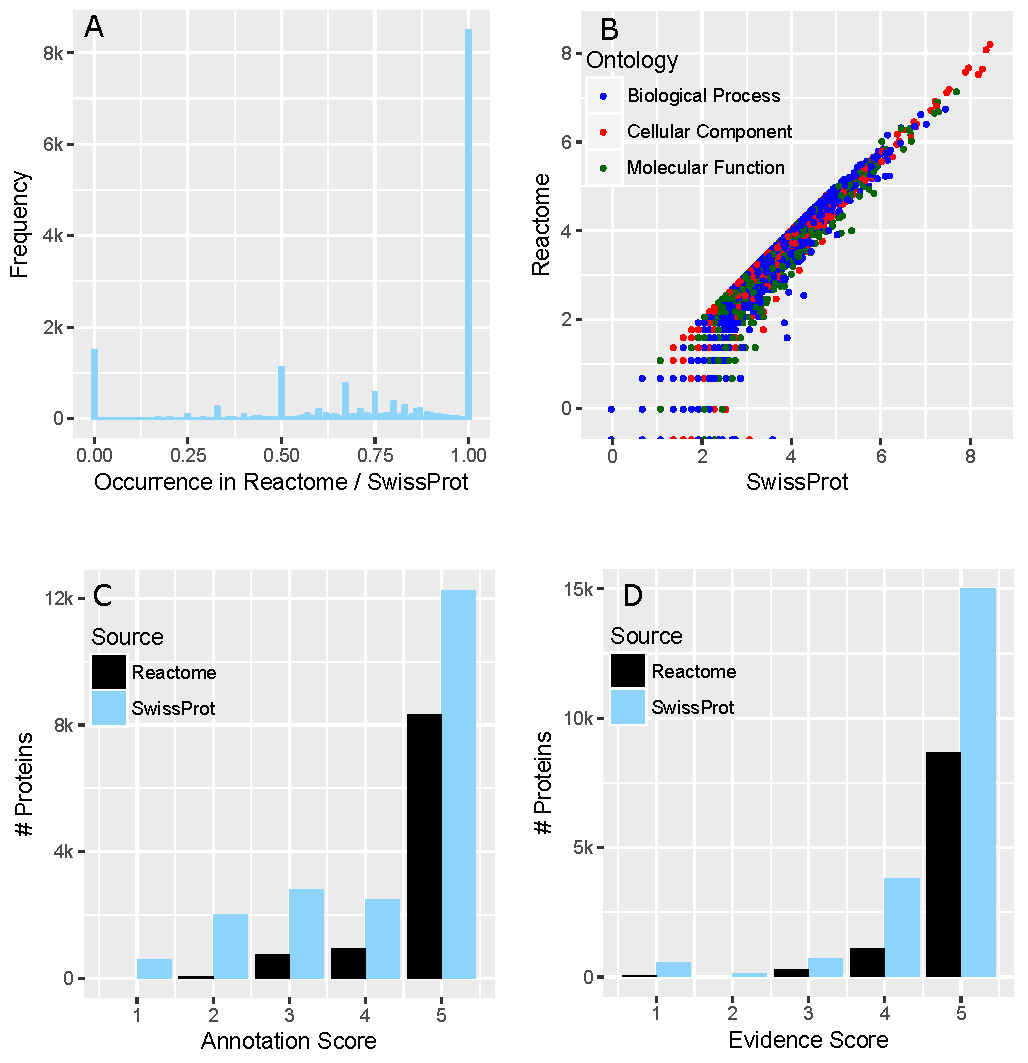
\includegraphics[width=\textwidth]{../S5/FigureS6.pdf}
  \caption{Potential biases in the curation process. Relative
    occurrence of GO terms (A and B) or protein annotations (C and D)
    in Reactome vs. SwissProt. A) The number of GO terms that occur
    with the relative amount indicated on the x-axis (bins of
    0.01). B) Each point indicates one GO term. The axes are
    log-scale, and terms not included in Reactome are plotted at the
    bottom of the plot. Red: Cellular Component; green: Molecular
    Function; blue: Biological Process. C) Distributions of annotation
    and D) evidence scores of proteins in SwissProt and
    Reactome. Higher scores indicate more annotation and better
    evidence. Reactome contains only about half of the proteins in
    SwissProt, hence the much lower bars in general for Reactome.}
  \label{fig:s6}
\end{figure}

\clearpage

\begin{table}[H]
  \centering
  \caption{The number of pathways a sub-pathway directly participates in. Only those sub-pathways that are directly part of more than two pathways are shown.}
  \begin{tabular}{lr}
    \toprule
    Pathway Name&	Parents\\\midrule
    RAF/MAP kinase cascade&	20\\
    PIP3 activates AKT signaling&	9\\
    DAG and IP3 signaling&	5\\
    TAK1 activates NFkB by phosphorylation and activation of IKKs complex&	4\\
    MAP kinase activation in TLR cascade&	4\\
    Spry regulation of FGF signaling&	4\\
    MyD88:Mal cascade initiated on plasma membrane&	3\\
\bottomrule
  \end{tabular}
  \label{tab:st1}
\end{table}

\end{document}
